\section{Date: 2026-11-01}
\noindent \textbf{Series ID: MRTSMPCSM44X72USN} 

\noindent This series is titled Retail Sales: Retail Trade and Food Services and has a frequency of Monthly. The units are Percent Change from Preceding Period and the seasonal adjustment is Not Seasonally Adjusted.The observation start date is 1992-02-01 and the observation end date is 2026-08-01.The popularity of this series is 7. \\ 

\noindent \textbf{Series ID: ATNHPIUS41660Q} 

\noindent This series is titled All-Transactions House Price Index for San Angelo, TX (MSA) and has a frequency of Quarterly. The units are Index 1995:Q1=100 and the seasonal adjustment is Not Seasonally Adjusted.The observation start date is 1984-07-01 and the observation end date is 2026-04-01.The popularity of this series is 1. \\ 

\subsection{Raw Regression}
\noindent Regresses the two series against each other directly. A significant result here can come just as easily from both series sharing a long-run trend as from any real relationship.

\begin{center}
\begin{tabular}{lclc}
\toprule
\textbf{Dep. Variable:}                 & value\_fred\_ATNHPIUS41660Q & \textbf{  R-squared:         } &     0.005   \\
\textbf{Model:}                         &             OLS             & \textbf{  Adj. R-squared:    } &    -0.002   \\
\textbf{Method:}                        &        Least Squares        & \textbf{  F-statistic:       } &    0.6811   \\
\textbf{Date:}                          &       Sun, 01 Nov 2026      & \textbf{  Prob (F-statistic):} &    0.411    \\
\textbf{Time:}                          &           17:19:26          & \textbf{  Log-Likelihood:    } &   -804.57   \\
\textbf{No. Observations:}              &               137           & \textbf{  AIC:               } &     1613.   \\
\textbf{Df Residuals:}                  &               135           & \textbf{  BIC:               } &     1619.   \\
\textbf{Df Model:}                      &                 1           & \textbf{                     } &             \\
\textbf{Covariance Type:}               &          nonrobust          & \textbf{                     } &             \\
\bottomrule
\end{tabular}
\begin{tabular}{lcccccc}
                                        & \textbf{coef} & \textbf{std err} & \textbf{t} & \textbf{P$> |$t$|$} & \textbf{[0.025} & \textbf{0.975]}  \\
\midrule
\textbf{const}                          &     195.0947  &        8.184     &    23.839  &         0.000        &      178.910    &      211.280     \\
\textbf{value\_fred\_MRTSMPCSM44X72USN} &       0.6157  &        0.746     &     0.825  &         0.411        &       -0.860    &        2.091     \\
\bottomrule
\end{tabular}
\begin{tabular}{lclc}
\textbf{Omnibus:}       & 14.744 & \textbf{  Durbin-Watson:     } &    0.015  \\
\textbf{Prob(Omnibus):} &  0.001 & \textbf{  Jarque-Bera (JB):  } &   17.203  \\
\textbf{Skew:}          &  0.858 & \textbf{  Prob(JB):          } & 0.000184  \\
\textbf{Kurtosis:}      &  2.736 & \textbf{  Cond. No.          } &     12.2  \\
\bottomrule
\end{tabular}
%\caption{OLS Regression Results}
\end{center}

Notes: \newline
 [1] Standard Errors assume that the covariance matrix of the errors is correctly specified.

\begin{figure}
\centering
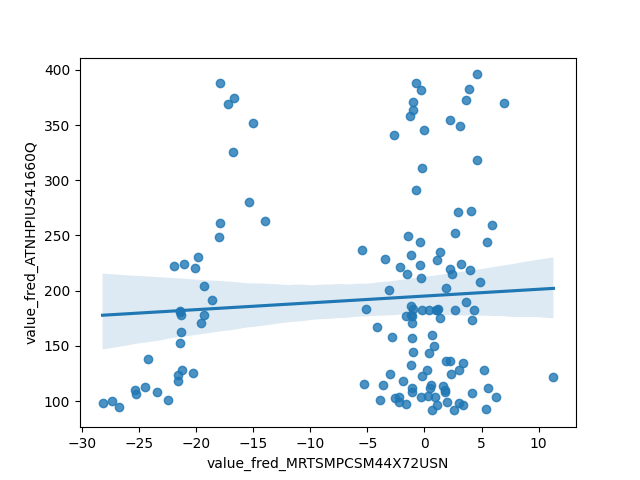
\includegraphics[scale = 0.9]{plots/plot_2026-11-01.png}
\caption{Raw Regression Plot for 2026-11-01}
\end{figure}
\newpage
\subsection{Detrended Regression}
\noindent Regresses the residuals of each series after removing its own linear time trend, so a shared trend can no longer drive the result on its own. A relationship that stays significant here is better evidence of a genuine link between the two series.

\begin{center}
\begin{tabular}{lclc}
\toprule
\textbf{Dep. Variable:}                            & value\_fred\_ATNHPIUS41660Q\_detrended & \textbf{  R-squared:         } &     0.004   \\
\textbf{Model:}                                    &                  OLS                   & \textbf{  Adj. R-squared:    } &    -0.004   \\
\textbf{Method:}                                   &             Least Squares              & \textbf{  F-statistic:       } &    0.5201   \\
\textbf{Date:}                                     &            Sun, 01 Nov 2026            & \textbf{  Prob (F-statistic):} &    0.472    \\
\textbf{Time:}                                     &                17:19:26                & \textbf{  Log-Likelihood:    } &   -646.65   \\
\textbf{No. Observations:}                         &                    137                 & \textbf{  AIC:               } &     1297.   \\
\textbf{Df Residuals:}                             &                    135                 & \textbf{  BIC:               } &     1303.   \\
\textbf{Df Model:}                                 &                      1                 & \textbf{                     } &             \\
\textbf{Covariance Type:}                          &               nonrobust                & \textbf{                     } &             \\
\bottomrule
\end{tabular}
\begin{tabular}{lcccccc}
                                                   & \textbf{coef} & \textbf{std err} & \textbf{t} & \textbf{P$> |$t$|$} & \textbf{[0.025} & \textbf{0.975]}  \\
\midrule
\textbf{const}                                     &   -3.134e-12  &        2.336     & -1.34e-12  &         1.000        &       -4.620    &        4.620     \\
\textbf{value\_fred\_MRTSMPCSM44X72USN\_detrended} &       0.1702  &        0.236     &     0.721  &         0.472        &       -0.296    &        0.637     \\
\bottomrule
\end{tabular}
\begin{tabular}{lclc}
\textbf{Omnibus:}       & 16.180 & \textbf{  Durbin-Watson:     } &    0.037  \\
\textbf{Prob(Omnibus):} &  0.000 & \textbf{  Jarque-Bera (JB):  } &   16.608  \\
\textbf{Skew:}          &  0.798 & \textbf{  Prob(JB):          } & 0.000248  \\
\textbf{Kurtosis:}      &  2.400 & \textbf{  Cond. No.          } &     9.90  \\
\bottomrule
\end{tabular}
%\caption{OLS Regression Results}
\end{center}

Notes: \newline
 [1] Standard Errors assume that the covariance matrix of the errors is correctly specified.

\begin{figure}
\centering
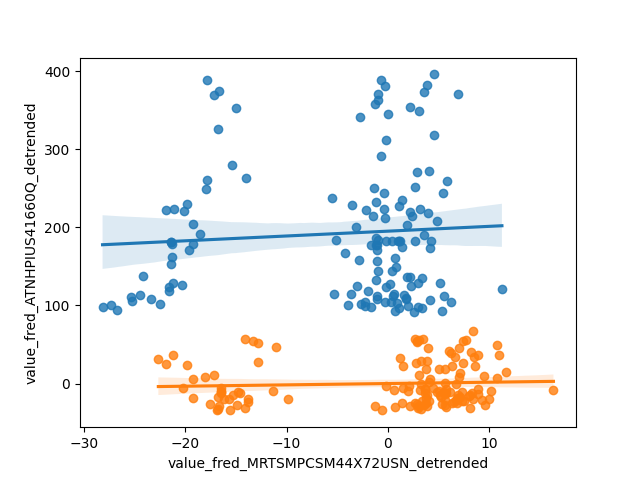
\includegraphics[scale = 0.9]{plots/plot_2026-11-01_detrended.png}
\caption{Detrended Regression Plot for 2026-11-01}
\end{figure}
\newpage
